\documentclass{article}
\usepackage[utf8]{inputenc}

\usepackage{graphicx}
\usepackage{subcaption}
\usepackage[export]{adjustbox}
\usepackage{wrapfig}
\usepackage{amsmath}
\usepackage{float}
\usepackage{biblatex}
\addbibresource{project.bib}

\title{Nonlinear Oscillating Pendulum}
\author{Ruizhizi Xue}
\date{May 2022}

\begin{document}
\maketitle

\begin{abstract}
    Starting from a simple pendulum model, use Newton’s second law for rotation to formulate an ordinary differential equation whose solution relates the string’s angle ($\theta$) to time ($t$). Extract the period of oscillation to construct Euler method with dimensionless time. Analyze the common results derived from solution of ODE and Euler method. Same procedure is conducted with involvement of drag force and a similar rod pendulum. The purpose of this project is to implement tools and methods learned from the Intro to Math Modeling course via exploring the factors involved in pendulum motion.
\end{abstract}

\tableofcontents


\section{Introduction}
\quad The classic model of pendulum has been studied for hundreds of years. Plentiful related resources has made this typical nonlinear oscillator model an ideal topic to examine the takeaways from the Math Modeling course. Let there be a point object with mass $m$ hanging on a string of length $l$. We first assume there is no drag force acting on it to investigate the influence of initial height on period and amplitude of motion. Then, consider real world scenario when air resistance as well as friction on the anchor play a role. It is expected to display the effect of different levels of drag force on the system. In addition, we are looking into a rod pendulum to compare its nature with a point pendulum.


\section{Model}

\subsection{Part 1}
Start with a dimensional analysis on a simple pendulum to find its period of oscillation ($\tau$). We know the dimensions
\[\tau=T,\quad g=\frac{L}{T^2}\quad \textrm{and}\quad l=L\]
so that \[\tau=L=\sqrt{\frac{L\cdot T^2}{L}}=\sqrt{\frac{l}{g}}\]
To get the equation of motion for the pendulum, we can use Newton's second law for rotation
\[\tau_q=I\alpha\]
where $\tau_q$ is torque, $I$ is moment of inertia, and $\alpha$ is angular acceleration. In this simple pendulum case,
\[\tau_q=rF=-mgl \cdot sin(\theta),\quad I=ml^2,\quad \alpha=\frac{d^2\theta}{dt^2}=\ddot{\theta}\]
so that
\begin{align*}
    -mgl \cdot sin(\theta) &= ml^2\ddot{\theta}\\
    \ddot{\theta}+\frac{g}{l}sin(\theta) &= 0
\end{align*}
For small $\theta$, by L'Hopital's rule,
\[\lim_{\theta\to 0}\frac{sin(\theta)}{\theta}=\lim_{\theta\to 0}\frac{cos(\theta)}{1}=1 \Rightarrow sin(\theta)\approx\theta\]
Therefore, for small deviation angles $\theta$, we can write
\begin{align*}
    \ddot{\theta}+\frac{g}{l}\theta &= 0\\
    \theta &= -\frac{l}{g}\ddot{\theta} \tag{1}
\end{align*}
With initial conditions $\theta(0)=\theta_0$ and $\dot{\theta}(0)=0$, the solution to the linear ODE is \[\theta=\theta_0 cos(\sqrt{\frac{g}{l}}t) = \theta_0 cos(\omega t)\] where $\omega=\sqrt{\frac{g}{l}}$ is the frequency of oscillation.
Indeed, \[\ddot{\theta}=-\theta_0\frac{g}{l}cos(\sqrt{\frac{g}{l}}t) \Rightarrow \theta = -\frac{l}{g}\ddot{\theta}\]
and $\tau=\frac{2\pi}{\omega}=2\pi\sqrt{\frac{l}{g}}$ confirming the result from dimensional analysis.

\subsection{Part 2}
By Euler method, approximate $\theta$ with the initial nonlinear ODE
\begin{align*}
    \ddot{\theta} &= -\frac{g}{l}sin(\theta)\\
    &\approx \frac{\dot{\theta}(t+\Delta t)-\dot{\theta}(t)}{\Delta t}\\
    &\approx \frac{\frac{\theta(t+2\Delta t)-\theta(t+\Delta t)}{\Delta t}-\frac{\theta(t+\Delta t)-\theta(t)}{\Delta t}}{\Delta t}\\
    -\frac{g}{l}sin(\theta_{i+1}) &= \frac{\theta_{i+2}-2\theta_{i+1}+\theta_i}{\Delta t^2}\\
    \theta_{i+2} &= -\frac{\Delta t^2 g}{l}sin(\theta_{i+1})-\theta_i+2\theta_{i+1} \tag{2}
\end{align*}

With $\theta(0)=\theta_0$ and $\dot{\theta}(0)=0$, set the initial terms of the Euler method to be \[\theta_0=\theta(0)=\theta_0\quad and\quad \theta_1=\theta(0)+\Delta t\cdot\dot{\theta}(0)=\theta_0\]
To generalize, use dimensionless time steps $\Delta t_d=\frac{\Delta t}{\tau}$ such that $\Delta t=\Delta t_d \cdot 2\pi\sqrt{\frac{l}{g}}$. Substitute into equation (2) to get
\[\theta_{i+2}=-4\pi^2 \Delta t_d^2 \cdot sin(\theta_{i+1})-\theta_i+2\theta_{i+1} \tag{3}\]
To cover three oscillation periods, let $\sum{}^{}\Delta t_d=3$. 
Simulating with $\theta_0=0.4$ and different step sizes $\Delta t_d$, we get
\begin{figure}[H]
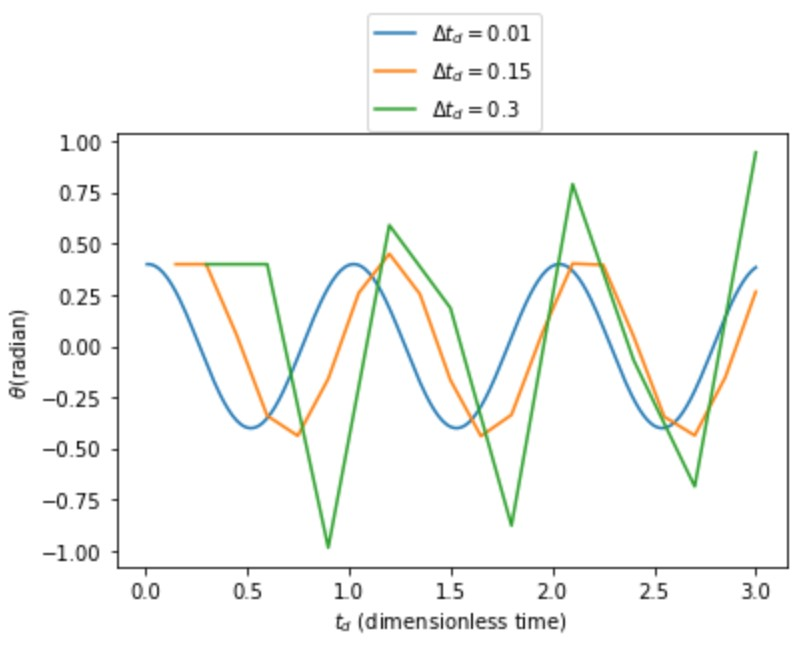
\includegraphics[width=4in]{SimpleEulerDifferentDeltaTd.jpg}
\caption{Euler method. Using different time steps to simulate pendulum motion}
\end{figure}
\noindent The figure shows that with large $\Delta t_d$, simulation becomes inaccurate as the amplitude of oscillation increases between cycles. Therefore, we choose a relatively small value $\Delta t_d=0.01$ to continue. Simulations for different initial positions $\theta_0$ is then
\begin{figure}[H]
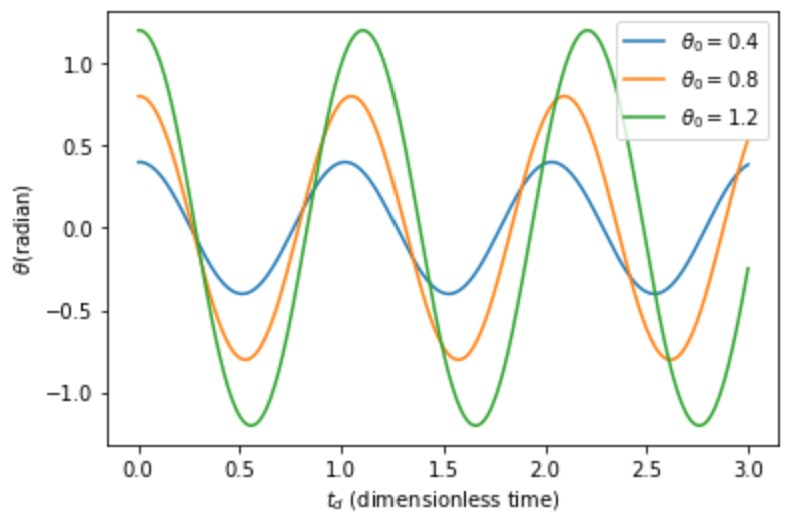
\includegraphics[width=4in]{SimpleEulerDifferentTheta0.jpg}
\caption{Euler method. Using different initial positions to simulate pendulum motion with dimensionless time step $\Delta t_d=0.01$}
\end{figure}
\noindent Replacing $\Delta t$ with dimensionless time $\Delta t_d$ in the analytical solution (1) in Part 1, we get
\[\theta=\theta_0\cdot cos(\sqrt{\frac{g}{l}}\cdot t_d \cdot 2\pi\sqrt{\frac{l}{g}})=\theta_0\cdot cos(2\pi t_d) \tag{4}\]
For different $\theta_0$, this function gives
\begin{figure}[H]
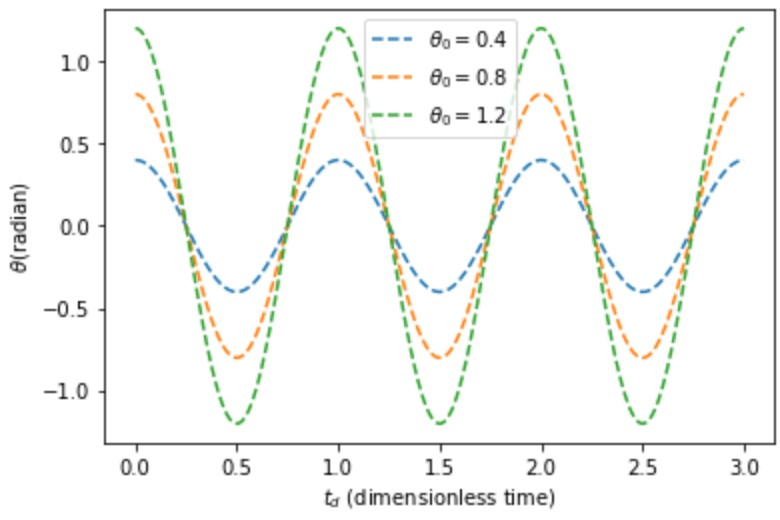
\includegraphics[width=4in]{SimpleAnalyticalDifferentTheta0.jpg}
\caption{Analytical solution from linear ODE.}
\end{figure}
\noindent Both methods show that the amplitude of oscillation decreases as the initial angle $\theta_0$ decreases. Indeed, intuitively, pendulum starting from a higher angle swings higher, since they possess more gravitational potential energy that does not reduce due to the absence of drag force.

\subsection{Part 3}
Now take drag force on the mass into consideration. It is practical to consider an object's drag force in fluid to be proportional to its velocity \[F_d=-kv\] where $k$ is a drag constant depending on properties of air(viscosity, density), properties of the object(shape, material) and so on. With linear acceleration $a=r\ddot{\theta}$ and linear velocity $v=r\dot{\theta}$, use Newton's second law of motion to get
\begin{align*}
    ma &= F+F_d\\
    ml\ddot{\theta} &= -mg\cdot sin(\theta)-kl\dot{\theta}\\
    \ddot{\theta} &= -\frac{g}{l}sin(\theta)-k\dot{\theta} \tag{5}
\end{align*}
To solve the equation\cite{Mohazzabi}, construct an auxiliary equation\cite{Stewart}
\[r^2+k r+\frac{g}{l}=0\]
which has solution
\[r=\frac{-k \pm \sqrt{k^2-4\frac{g}{l}}}{2}\]
Since air resistance is small \footnote{To be honest this is because I find it too hard to compute the other two conditions when $b^2-4ac$ is $0$ or positive.}, assume that $k^2<4\frac{g}{l}$ so that 
\[r=\frac{-k \pm i\sqrt{4\frac{g}{l}-k^2}}{2}\]
\[r_1=-\frac{k}{2}+i\sqrt{\frac{g}{l}-\frac{k^2}{4}},\quad r_2=-\frac{k}{2}-i\sqrt{\frac{g}{l}-\frac{k^2}{4}}\]
As a result, the solution to the differential equation is 
\[\theta=e^{-\frac{k}{2}t} (c_1\cdot cos(\omega t)+c_2 \cdot sin(\omega t)) \tag{6}\]
where $\omega=\sqrt{\frac{g}{l}-\frac{k^2}{4}}$, the imaginary part of the roots, is also the angular frequency of the pendulum. Substitute with initial conditions $\theta(0)=\theta_0$ and $\dot{\theta}(0)=0$, we can get
\[c_1=\theta_0\]
and 
\begin{align*}
    -\frac{k}{2}\theta_0+\omega c_2 &= 0\\
    c_2 &= \frac{k\theta_0}{2\omega}
\end{align*}
Replace $c_1$, $c_2$ in (6), we get the function for $\theta$
\[\theta=\theta_0 e^{-\frac{k}{2}t} (cos(\omega t)+\frac{k}{2\omega} \cdot sin(\omega t)) \tag{7}\]
Similar to the process in Part 1, Euler method provides the equation
\begin{align*}
    -\frac{g}{l}sin(\theta)-k\cdot \frac{\theta_{i+1}-\theta_i}{\Delta t} &= \frac{\theta_{i+2}-2\theta_{i+1}+\theta_i}{\Delta t^2}\\
    -\Delta t^2\frac{g}{l}sin(\theta_{i+1})-\Delta t k(\theta_{i+1}-\theta_i) &= \theta_{i+2}-2\theta_{i+1}+\theta_i\\
    (\Delta t k-1)\theta_i-\Delta t^2 \frac{g}{l}sin(\theta_{i+1})+(2-\Delta t k)\theta_{i+1} &= \theta_{i+2} \tag{8}
\end{align*}
Again, use dimensionless time $\Delta t_d=\frac{\Delta t}{\tau}$ where $\tau=\frac{2\pi}{\omega}$. Since the length of the string is unknown, we assume for simplicity $l=g$, so that $\omega=\sqrt{1-\frac{k^2}{4}}$. In this case, (8) becomes
\[\theta_{i+2}=(\Delta t_d \tau k-1)\theta_i-\Delta t_d^2 \tau^2 sin(\theta_{i+1})+(2-\Delta t_d \tau k)\theta_{i+1} \tag{9}\]
Try using different dimensionless time step sizes with $\theta_0=0.4$ and drag constant $k=0.5$, we get
\begin{figure}[H]
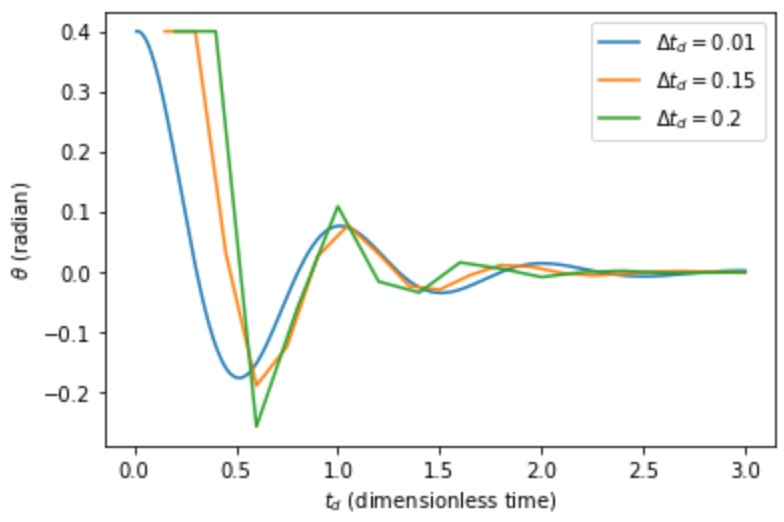
\includegraphics[width=4in]{DragEulerDifferentDeltaTd.jpg}
\caption{Euler method. Using different time steps to simulate pendulum motion with fixed $k=0.5$ and $\theta_0=0.4$}
\end{figure}
\noindent To get a smooth curve with more consistent amplitude, continue with a relatively small step size $\Delta t_d=0.01$. Simulations for different initial positions is then 
\begin{figure}[H]
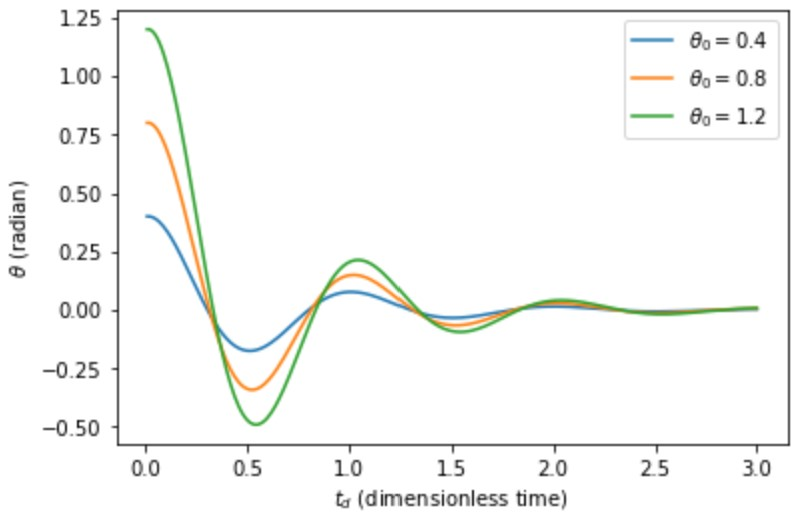
\includegraphics[width=4in]{DragEulerDifferentTheta0.jpg}
\caption{Euler method. Using different initial positions to simulate pendulum motion with $k=0.5$}
\end{figure}
\noindent Again, masses starting from higher angles oscillate with larger amplitudes, as they possess more gravitational potential energy. It also takes longer for the drag force to settle them down.\\
To compare with the analytical solution, same parameters are used to graph function (7). The results are approximately the same.
\begin{figure}[H]
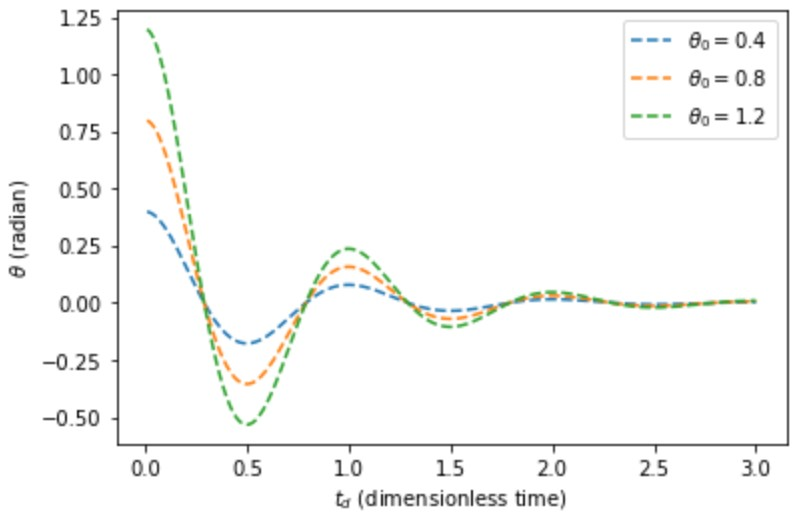
\includegraphics[width=3.9in]{DragAnalyticalDifferentTheta0.jpg}
\caption{Analytical solution from nonlinear ODE}
\end{figure}
\noindent To test out the effect of drag force, fix $\theta_0=0.4$ and try different drag constants. Follow the previous assumption \[k^2<4\frac{g}{l}=4 \Rightarrow k<2\]
Euler method shows
\begin{figure}[H]
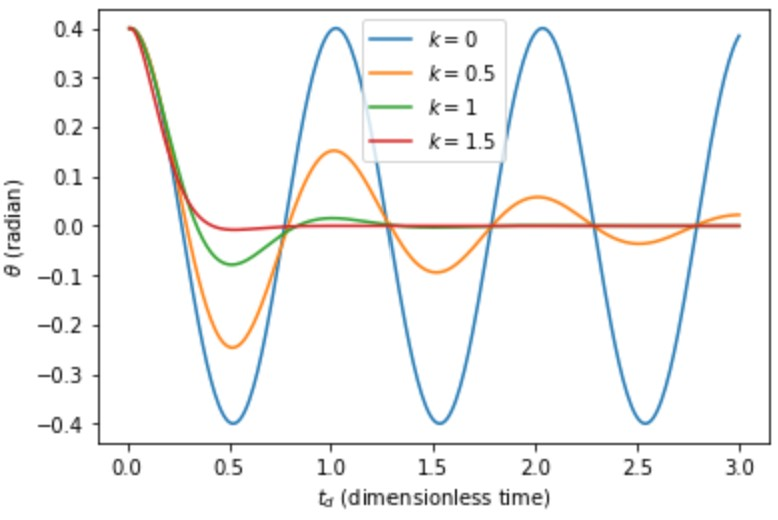
\includegraphics[width=4in]{DragEulerDifferentK.jpg}
\caption{Euler method. Fix $\theta_0=0.4$ to test different $k$}
\end{figure}
\noindent Analytical solution shows approximately the same result
\begin{figure}[H]
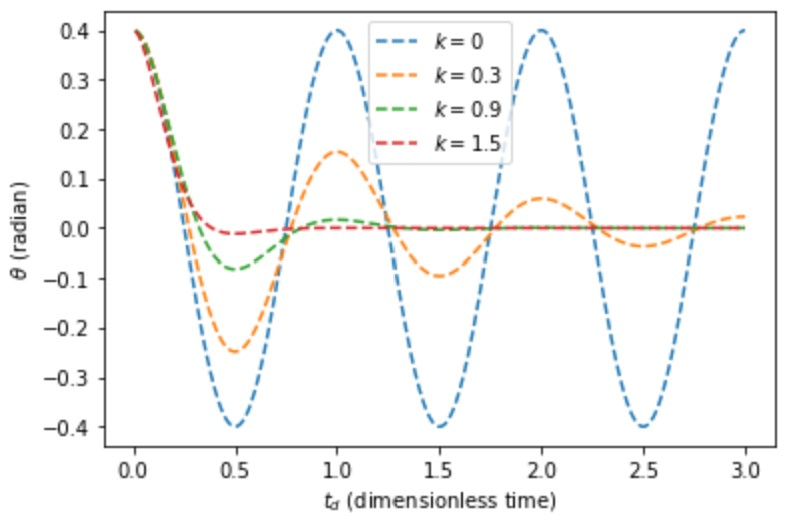
\includegraphics[width=4in]{DragAnalyticalDifferentK.jpg}
\caption{Analytical solution for different $k$}
\end{figure}
\noindent The figures show that when $k=0$, there is no drag force so that the pendulum swings indefinitely. As $k$ increases, amplitude of oscillation decays faster. With extremely large $k$, possibly $k>2$, the pendulum could stop within few periods, even within one. The plots of angle $\theta$ versus angular velocity $\alpha$ also confirms this statement.
\begin{figure}[H]
\begin{subfigure}{0.5\textwidth}
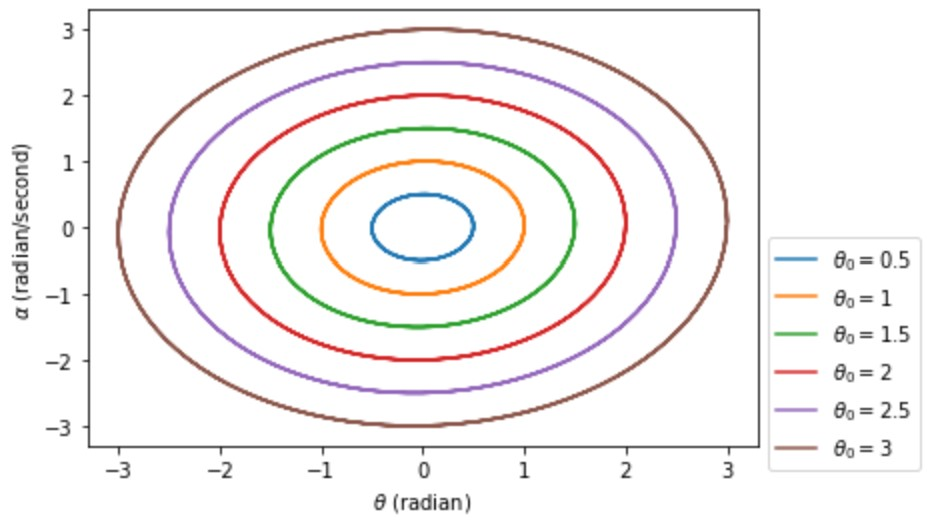
\includegraphics[width=0.9\linewidth, height=5cm]{AlphaThetaK0.jpg} 
\caption{$k=0$}
\label{fig:subim1}
\end{subfigure}
\begin{subfigure}{0.5\textwidth}
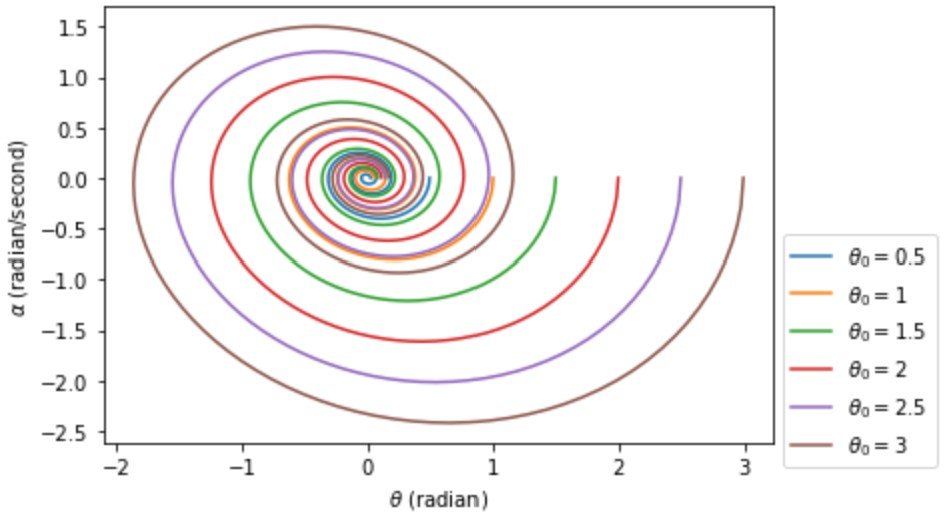
\includegraphics[width=0.9\linewidth, height=5cm]{AlphaThetaK03.jpg}
\caption{$k=0.3$}
\label{fig:subim2}
\end{subfigure}
\begin{subfigure}{0.5\textwidth}
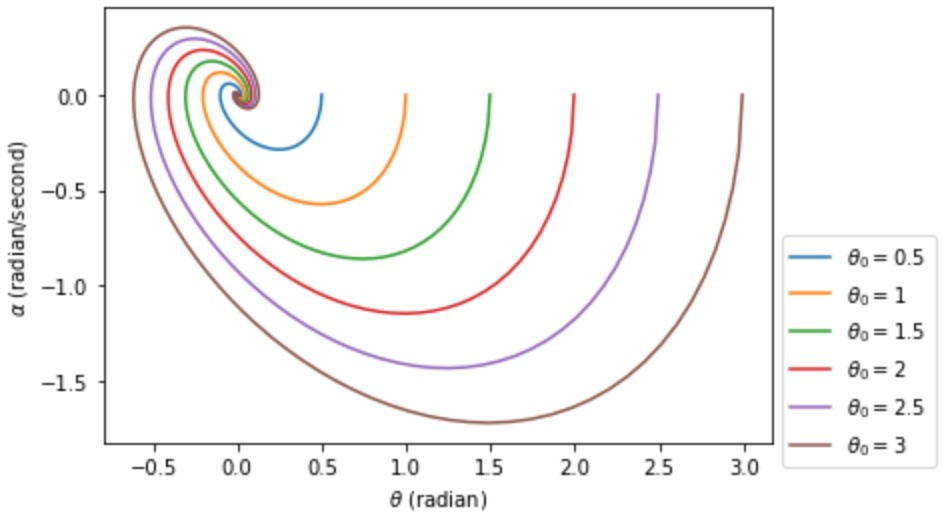
\includegraphics[width=0.9\linewidth, height=5cm]{AlphaThetaK09.jpg} 
\caption{$k=0.9$}
\label{fig:subim3}
\end{subfigure}
\begin{subfigure}{0.5\textwidth}
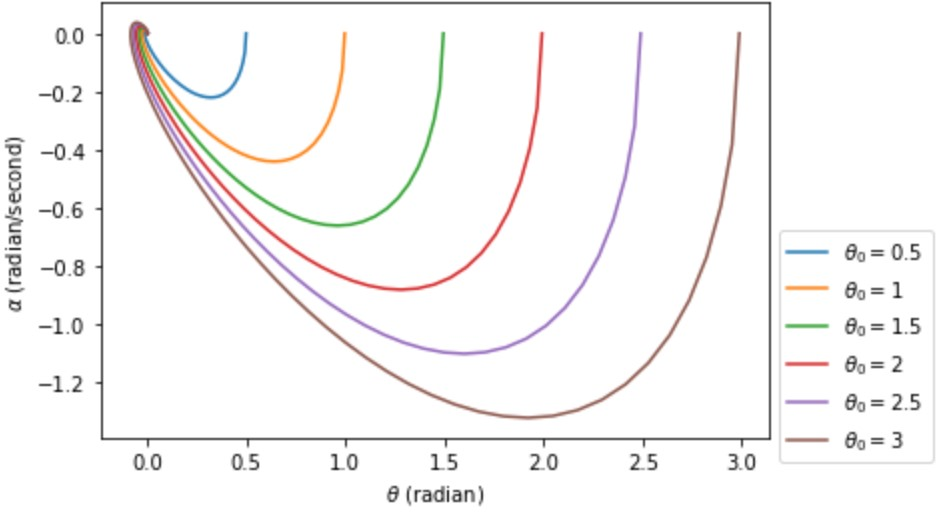
\includegraphics[width=0.9\linewidth, height=5cm]{AlphaThetaK15.jpg}
\caption{$k=1.5$}
\label{fig:subim4}
\end{subfigure}
\caption{$\alpha$ (i.e. $\dot{\theta}$) versus $\theta$ for different drag constants and different initial angles}
\label{fig:image1}
\end{figure}
\noindent In sub-figure (a), since no friction, the non-stop pendulum never reaches the origin. In the other three sub-figures, as k increases, the pendulum reaches origin in less number of periods.

\subsection{Part 4}
Now the mass is no longer a point object, but a rod with mass $m$ and length $l$. Consider each point (or indefinitely small segment) on the rod, let $x$ be the distance between the anchor and the point, then we have its linear velocity \[v=\dot{\theta}\cdot x\]
so that its drag force is \[F_{d,x}=-k\dot{\theta}x\]
Also, the mass on the point can be regarded as \[m_x=\frac{m}{l}\]
such that its gravitational force is \[G_x=-g\frac{m}{l}sin(\theta)\]
The torque (denote as $\tau_q$ to distinguish from previous notation) on this point is therefore
\begin{align*}
    \tau_{q, x} &= x \cdot (F_{d,x}+G_x)\\
    &= -g\frac{m}{l}sin(\theta)\cdot x-k\dot{\theta}x^2
\end{align*}
Integrate to get the torque for the entire rod
\begin{align*}
    \tau_q &= \int_{0}^{l} (-g\frac{m}{l}sin(\theta)\cdot x-k\dot{\theta}x^2) \,dx\\
    &= -\frac{1}{2}mgl\cdot sin(\theta)-\frac{1}{3}k\dot{\theta}l^3
\end{align*}
By Newton's second law for rotation, 
\[\tau_q=-\frac{1}{2}mgl\cdot sin(\theta)-\frac{1}{3}k\dot{\theta}l^3=I\ddot{\theta} \tag{10}\]
where it is known that the moment of inertia for a rotating rod is
\[I=\frac{1}{3}ml^2\]
Substitute into (10), we can get the equation of motion
\[\ddot{\theta}=-\frac{3g}{2l}sin(\theta)-\frac{k\dot{\theta}l}{m} \tag{11}\]
which is quite alike to equation (5) in Part 3. I foresee a similar but a little more complicated process that is painful to go through again. So I decide to stop here ;-;.


\section{Discussion}
\quad With reasonably small time step, in our case one percent of oscillation period, Euler method can accurately approximate the actual state of motion.

In all cases, we have shown that the frequency and period of motion is related to string length $l$ and drag constant $k$, but not the mass' initial position $\theta_0$. $\theta_0$ decides the gravitational potential energy within the object, so that higher initial angle corresponds with higher velocity and amplitude due to conservation of energy. Larger drag constant $k$ implies stronger friction, which takes the pendulum faster into rest state.


\section{Conclusion}
\quad This project implemented mathematical techniques such as solving ordinary differential equations and Euler method to reveal the nature of pendulum. The results are indeed intuitive in real life, in compliance with the universal principles of physics.

\printbibliography

\end{document}
